\subsection{Opgave 27}

En jernklods opvarmes og afkøles derefter af luften i lokalet. Afkølingen kan beskrives af funktionen

\begin{align*}
    a(t) = 20 + 880\cdot 0,95^t, t\geq 0
\end{align*}

hvor afkølingen påbegyndes til $t=0$ og $a(t)$ er klodsens temperatur målt i $^{\circ}C$ til tiden $t$, målt i minutter.

a) Tegn grafen for funktionen.

\ans
For at tegne grafen for funktionen kan vi opstille et sildeben for t værdierne 0, 3, 6, 9, 12.

\begin{tabular}{c|c|c|c|c|c}
    t & 0 & 3 & 6 & 9 & 12 \\\hline
    $a(t)$ & & & & &
\end{tabular}

Vi beregner nu $a(t)$ for de forskellige t værdier i sildebenet

\begin{align*}
    a(0) &= 20 + 880 \cdot 0.95^0 = 900.00 \\
    a(3) &= 20 + 880 \cdot 0.95^3 = 774.49 \\
    a(6) &= 20 + 880 \cdot 0.95^6 = 666.88 \\
    a(9) &= 20 + 880 \cdot 0.95^9 = 574.62 \\
    a(12) &= 20 + 880 \cdot 0.95^{12} = 495.52
\end{align*}

Udfylder vi sildebenet får vi

\begin{tabular}{c|c|c|c|c|c}
    t & 0 & 3 & 6 & 9 & 12 \\\hline
    $a(t)$ & 900 & 774,49 & 666,88 & 574,62 & 495,52
\end{tabular}

Nu kan vi så tage hver kolonne i sildebenet og indsætte dem som punkter i et koordinatsystem.
Den første kolonne svarer altså til punktet (0, 900) den næste kolonne til punktet (3, 774,49) osv.
Indsætter nu punkterne i et koordinatsystem og forbinder dem med en linje.
Den indtegnede funktion kan ses på billedet nedenfor.

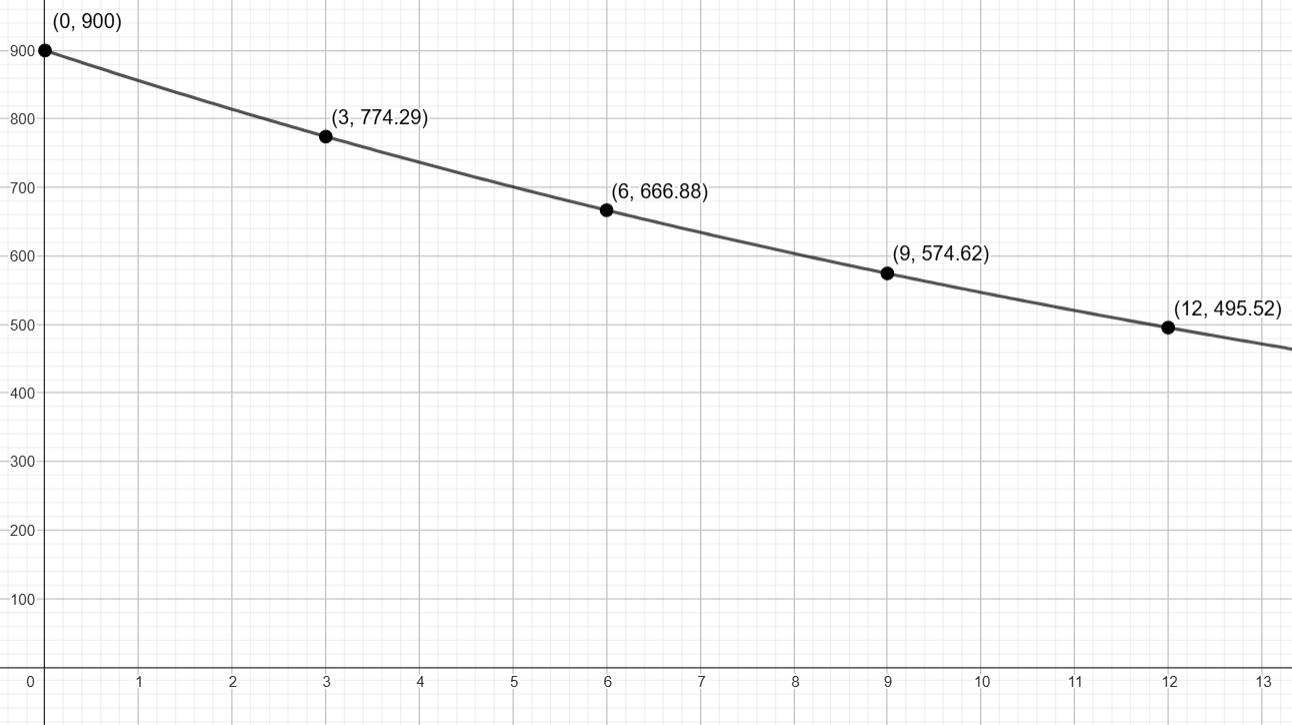
\includegraphics[width=10cm]{Opgave_21-30/Opgave_27/27.png}


b) Bestem $a(15)$

\ans
For at bestemme $a(15)$ bruger vi funktionen $a(t)$ og indsætter $t=15$. 
Vi beregner og får
\begin{align*}
    a(15) = 20 + 880\cdot 0,95^{15} = 427,70 
\end{align*}

Det betyder at efter $t = 15$ minutter er klodsens temperatur $a(15) = 427,70$ grader celcius. 

